% !TEX encoding = UTF-8 Unicode
\documentclass[a4paper]{article}

\usepackage{color}
\usepackage{url}
\usepackage[T2A]{fontenc} % enable Cyrillic fonts
\usepackage[utf8]{inputenc} % make weird characters work
\usepackage{graphicx}
\usepackage[margin=1.5in]{geometry}
\usepackage[table]{xcolor}

\usepackage[english,serbian]{babel}
%\usepackage[english,serbianc]{babel} %ukljuciti babel sa ovim opcijama, umesto gornjim, ukoliko se koristi cirilica

\usepackage[unicode]{hyperref}
\hypersetup{colorlinks,citecolor=green,filecolor=green,linkcolor=blue,urlcolor=blue}

\usepackage{listings}
\renewcommand\lstlistingname{Kod}
\renewcommand\lstlistlistingname{Kodovi}

%\newtheorem{primer}{Пример}[section] %ćirilični primer
\newtheorem{primer}{Primer}[section]

\definecolor{mygreen}{rgb}{0,0.6,0}
\definecolor{mygray}{rgb}{0.5,0.5,0.5}
\definecolor{mymauve}{rgb}{0.58,0,0.82}

\lstset{ 
  backgroundcolor=\color{white},   % choose the background color; you must add \usepackage{color} or \usepackage{xcolor}; should come as last argument
  basicstyle=\scriptsize\ttfamily,        % the size of the fonts that are used for the code
  breakatwhitespace=false,         % sets if automatic breaks should only happen at whitespace
  breaklines=true,                 % sets automatic line breaking
  captionpos=b,                    % sets the caption-position to bottom
  commentstyle=\color{mygreen},    % comment style
  deletekeywords={...},            % if you want to delete keywords from the given language
  escapeinside={\%*}{*)},          % if you want to add LaTeX within your code
  extendedchars=true,              % lets you use non-ASCII characters; for 8-bits encodings only, does not work with UTF-8
  firstnumber=1,                % start line enumeration with line 1000
  frame=single,	                   % adds a frame around the code
  keepspaces=true,                 % keeps spaces in text, useful for keeping indentation of code (possibly needs columns=flexible)
  keywordstyle=\color{blue},       % keyword style
  language=Python,                 % the language of the code
  morekeywords={*,...},            % if you want to add more keywords to the set
  numbers=left,                    % where to put the line-numbers; possible values are (none, left, right)
  numbersep=5pt,                   % how far the line-numbers are from the code
  numberstyle=\tiny\color{mygray}, % the style that is used for the line-numbers
  rulecolor=\color{black},         % if not set, the frame-color may be changed on line-breaks within not-black text (e.g. comments (green here))
  showspaces=false,                % show spaces everywhere adding particular underscores; it overrides 'showstringspaces'
  showstringspaces=false,          % underline spaces within strings only
  showtabs=false,                  % show tabs within strings adding particular underscores
  stepnumber=2,                    % the step between two line-numbers. If it's 1, each line will be numbered
  stringstyle=\color{mymauve},     % string literal style
  tabsize=2,	                   % sets default tabsize to 2 spaces
  title=\lstname                   % show the filename of files included with \lstinputlisting; also try caption instead of title
}

\begin{document}

\title{Debagovanje u LLDB-u\\ \small{Seminarski rad u okviru kursa\\Metodologija stručnog i naučnog rada\\ Matematički fakultet}}

\author{Momir Adžemovic, Miloš Miković, Marko Spasić,\\ Mladen Dobrašinović\\ \\ \small momir.adzemovic@gmail.com, spaskeasm@gmail.com,\\ \small milos.mikovicpos@gmail.com, dobrasinovic.mladen@gmail.com}

\date{1.~april 2020.}

\maketitle

\abstract{
Ovaj rad predstavlja grupni projekat u okviru kursa Metologija stručnog i naučnog rada. Ovo je dobra prilika da podelimo sa kolegama naša znanja koja smo stekli ovim istraživanjem koje ima velike primene u praksi. Rad većinom pokriva interesatne informacije o debageru LLDB kao jednom od produžetaka LLVM-a, način korišćenja LLDB i poređenje sa ostalim debagerima.  

}

\tableofcontents

\newpage

\section{Uvod}
\label{sec:uvod}

U vreme pisanja ovog rada broj dostupnih debagera za najpopularnije programske jezike meri se u desetinama. Svaki sa svojim specifičnostima koji variraju od platforme do platforme. Za programske jezike C, C++, Objective-C najpopularniji izbori su LLDB, GDB i Microsoft Visual Studio debager. Nije na prvi pogled očigledno koji je najbolji u zavisnosti od projekta na kom se radi niti zašto bi neko ko tek počinje svoju karijeru uopšte koristio alat kao što je debager.
Nakon pročitanog rada čitalac će biti upoznat sa osnovnim tehnikama debagovanja i specifičnostima debagovanja sa LLDB-om. Za one kojima više odgovara rad u integrisanom razvojnom okruženju poglavlje \ref{sec:Koja razvojna okruzenja podrzavaju upotrebu ovog debagera i kako?} daje pregled popularnih razvojnih okruženja i na koji način integrišu LLDB. Na kraju, predstavljena su poređenja LLDB-a sa drugim debagerima kako bi čitalac lakše mogao da donese odluku da li je LLDB pravi izbor za posao kojim se bavi u zavisnosti od platforme na kojoj radi. 


% Milosev deo
\section{Šta je debagovanje}
\label{sec:sta je debagovanje}

Debagovanje je proces identifikacije pravog problema i njegovo ispravljanje.
“Debagovanje je duplo teže od kodiranja, ako napišete kod na najlukaviji (odnosno najkomplikovaniji) način, po definiciji niste dovoljno pametni da ga debagujete. ( Brian w. Keringhan) \cite{debagovanje_vladaf}\\
Koraci pri debagovanju\cite{bagovi_smalkov}:
\begin{enumerate}
\item uočavanje da postoji greška
\item razumevanje greške
\item lociranje greške
\item ispravljanje greške
\end{enumerate}
Često je najteži deo ispravno razumevanje i rano otkrivanje greške, kada se greška locira, ispravljanje najčešće nije veliki problem.


\subsection{Bagovi uopšteno}
\label{subsec:podnaslov1}

Postojanje grešaka (bagova) se često neopravdano poistovećuje sa propustima u programiranju.
U širem kontekstu bag, greška, defekt ili propust se odnosi na bilo koju vrstu problema u bilo kojoj fazi procesa razvoja kao što su greške u projektovanju, planiranju, arhitekturi, dizajnu…
Zato se često termini propust i greška koriste u širem kontekstu razvoja a termin bag u užem i vezan je za propuste u programiranju.\\
\indent Jedna od najčešćih klasifikacija bagova prema načinu ispoljavanja obuhvata:
\begin{enumerate}
	\item \textbf{Nekonzistentnosti u korisničkom interfejsu}: često je slučaj da se komanda ctr+f koristi za pretraživanje dokumenta, Outlook koristi   
	tu komandu za prosleđivanje poruke
	\item \textbf{Neispunjena očekivanja}: dobijanje neočekivanog (pogrešnog) rezultata
	\item \textbf{Slabe performanse}: stalno ili povremeno čekanje rezultata zbog lošeg odziva sistema, takvi programi su često ne upotrebljivi
	\item \textbf{Padovi sistema i oštećenja podataka}: predstavljaju najopasniji vid bagova, mogu trajno oštetiti sistem i podatke
\end{enumerate}
\indent Bagovi su jako neugodni i treba ih sistematski otklanjati čestim refaktorisanjem i planskim gradjenjem koda. Jedne od okolnosti koje pogoduju nastajanju bagova su nedovoljna stručnost razvojnog tima i povećan stres na poslu, a informisanost, sistematičnost i redovnost ih suzbijaju. \cite{bagovi_smalkov}

\begin{figure}[h!]
	\begin{center}
		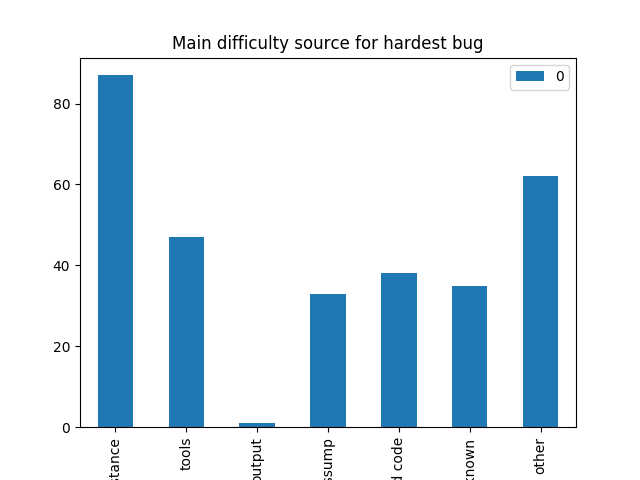
\includegraphics[width=100mm,height=50mm]{Slike/bagovi.png}
	\end{center}
	\caption{Glavni razlozi najtežih bagova\cite{study_bugs}}
	\label{fig:bagovi}
\end{figure}

Sa slike (\ref{fig:bagovi}) vidimo da su nejčešći razlozi za teške bagove upravo rastojanje od izvora greške do neočekivanog ponašanja. U ovim situacijama su veoma bitne metode debagovanja, pa i alati koji se koriste za debagovanje (debageri).

\subsection{Metode debagovanja}
\label{subsec:podnaslov2}

\begin{enumerate}
	\item \textbf{Neformalno debagovanje}: Neformalno debagovanje predstavlja jednostavan i površan pristup i čine ga dva koraka.
	\begin{enumerate}
		\item Pokušati sa nekom jednostavnom popravkom;
		\item Ponavljati korak (a) dok se problem ne reši.
	\end{enumerate}
	Ovaj metod se ne preporučuje u praksi i često može da proizvede nove probleme, pogotovo ako vršimo puno sitnih popravki za koje nismo sigurni da će rešiti problem. Ponekad, ako su u pitanju sitne greške, ovaj metod se može oprezno koristiti jer dovodi do brzog rešenja problema.\cite{bagovi_smalkov}
	
	\item \textbf{Empirijski naučni metod}:
	Ovaj postupak je sličan uobičajenom istaživačkom metodu u prirodnim naukama.
	Čine ga sledeći koraci:
	\begin{enumerate}
		\item Posmatrati uočen problem;
		\item Postaviti hipoteze o uzroku problema;
		\item Na osnovu hipoteza napraviti predviđanje ponašanja;
		\item Eksperimentalno proveriti ispravnost predviđanja;
		\item Ponavljati prethodne korake uz popravljanje ili menjanje hipoteze, sve dok se ne potvrdi ispravnost hipoteze ili ne ponestanu mogućnosti za njeno dalje unapređivanje.
	\end{enumerate}
	\indent Uopšteno gledano ovo je najbolji pristup debagovanju. Često je jako zahtevan i oduzima dosta vremena ali je sa druge strane je temeljan i koncizan.\cite{bagovi_smalkov}
	
	
	\item \textbf{Heurističko debagovanje}:
	Ova vrsta debagovanja podrazumeva postojanje heuristike (skup pravila) koja olakšava brže i efikasnije pronalaženje grešaka. Često se za određene skupove problema prave različite heuristike, koje se testiraju u praksi i kasnije koriste kao pravila pri otklanjanju određenih vrsta bagova. Ovakve heuristike odlikuje izbegavanje pravljenja previda pri posmatranju, sužavanje skupa kandidata za iskazivanje hipoteza, usmeravanje posmatranja prema uzroku problema i drugo.Heuristike nisu optimalna rešenja niti egzaktna pravila koja vode rešenju problema, ali često su jako efikasne i daju “dovoljno dobra rešenja”.\cite{bagovi_smalkov}
\end{enumerate}

\subsection{Tehnike za prevenciju bagova}
\label{subsec:Tehnike za prevenciju bagova}

Tehnike za prevenciju bagova mogu biti unutrašnje i spoljašnje. Unutrašnje predstavljaju sve ono što se ugrađuje u programski kod samo radi pomoći u prevenciji i otklanjanju grešaka. Neke od njih su pravljenje pretpostavki(asserts), komentarisanje značajnih odluka i mesta u kodu, testiranje jedinica koda... Spoljašnje tehnike i alati se koriste pri razvoju i ne ugrađuju se nužno u programski kod, ali se koriste u čitavom razvojnom ciklusu. Neki od spoljašnjih alata su debager, alati za praćenje verzija programskog koda, alati za podršku i praćenje komunikacije, alati za automatizovanje pravljenja dokumentacije\cite{bagovi_smalkov}.
\\

\begin{lstlisting}[language=C,caption=Primer korišćenja assert naredbe]
void example(int* ptr) {
assert (ptr != NULL);
printf ("%d\n",(ptr));
}
\end{lstlisting}


\subsection{Debager}
\label{subsec:Debager}

Debager je računarski program koji se koristi za uklanjanje grešaka, testiranje rada i proveru ispravnosti drugih programa. Debageri daju napredne funkcije kao što su pokretanje programa korak po korak (single-stepping), praćenje vrednosti promenjivih kao i stek okvira, praćenje na nivou instrukcija i stanja procesora, zaustavljanje ili pauziranje izvršavanja programa na takozvanim tačkama prekida (breakpoint), a neki čak i omogućavaju menjanje programa tokom izvršavanja.\\
\indent Većina popularnih debagera daje samo jednostavno komandno-linijsko okruženje (command-line interface - CLI), često iz razloga da maksimizuju portabilnost i minimizuju trošenje sistemskih resursa računara. Ipak, popravljanje grešaka u programu preko grafičkog korisničkog okruženja (GUI) debagera se često smatra jednostavnijim, produktivnijim i ugodnijim za rad. Neki debageri pružaju i mogućnosti obrnutog debagovanja (debagovanje unazad) koje omogućava da se vratimo na prethodno stanje programa (Step Beckward). Jedan od debagera koji pruža ovu mogućnost je IntelliTrace koji se koristi u Microsoft-ovom razvojnom okruzenju VisualStudio. Debagovanje unazad je jako korisno i sve se više koriste debageri koji omogućavaju ovo svojstvo. Mana debagovanja unazad je usporavanje čitavog procesa debagovnja pa čak i do dva puta. Debageri mogu biti zavisni od programskog jezika, ako se mogu koristiti za debagovanje jednog konkretnog jezika ili mogu biti višejezični i koristiti se za debagovanje više programskih jezika. Neki debageri uključuju i zaštitu memorije kako bi izbegli prekoračenje bafera, ili onemogućili korisnika da pristupa memoriji za koju nema dozvolu i slično.\cite{ssq_debug_def}

\subsection{Lista debagera}
\label{sec:Lista debagera}

Najčešće korišćeni debageri za  C, C++, Objective-C\cite{ll_best_debuggers}\cite{up_best_debuggers}:
\begin{enumerate}
	\item GDB(gnu debuger)
	\item DDD 
	\item Lldb
	\item Valgrind
	\item Nemiver
	\item Electric Fence
	\item Dbx
\end{enumerate}

% Mladenov deo
\section{Upoznavanje sa LLDB-om}
LLDB podržava standardne funkcije debagovanja preko komandne linije i može se
koristiti kao debager u interaktivnom razvojnom okruženju. Konkretno, sa
debagerom pokrenutim nad programom prevedenim sa debag opcijama omogućava
se \cite{lldb_to_gdb_map}:

\begin{itemize}
	\item{Aktiviranje procesa programa sa određenim argumentima komandne linije
		(eng. command line arguments).}
	
	\item{Korišćenje breakpoint-a (određenog reda ili funkcije u izvornom kodu pri
		kojima debager zaustavlja izvršavanje programa kada se stigne do odgovarajućeg
		dela izvršnog koda).}
	
	\item{Korišćenje watchpoint-a (određene promenljive, takve da debager zaustavlja
		proces ili nit kada se njeno stanje promeni).}
	
	\item{Korišćenje dodatnih uslova nad breakpoint-ovima i watchpoint-ovima.}
	\begin{itemize}
		\item{Nastavljanje ili pokretanje programa.}
	\end{itemize}
	
	\item{Pokretanje procesa red po red (sa ,,ulaženjem'' u funkciju ili bez).}
	
	\item{Istraživanje promenljivih ili memorije procesa.}
	
	\item{Izvršavanje proizvoljnog izraza nad stanjem procesa (npr. menjanje neke
		promenljive na steku).}
	
	\item{Istraživanje steka okvira poziva.}
	
	\item{Izvršavanje drugih naprednih i raznih funkcija.}
\end{itemize}

LLDB omogućava korišćenje eksternih skripti za debagovanje
preko javnog API-a za Python, izršavanje proizvoljnog Python koda unutar
debagera \cite{lldb_python} (preko ugnježdenog interpretatora (eng. embedded
interpreter) i omogućavanje REPL (Read-Evaluate-Print-Loop) funkcija za
programske jezike zajedno sa mogućnostima debagovanja \cite{swift_lldb_repl}.

\subsection{LLDB interfejs komandne linije}
LLDB interfejs komandne linije (eng. command line interface) se aktivira pozivom
\verb|lldb| u komandnoj liniji (eng. shell) sa argumentom koji predstavlja program koji
će biti debagovan. Program komandne linije \verb|lldb| se odlikuje struktuisanom sintaksom
osnovnih komandi koja je sledećeg oblika \cite{lldb_tutorial}:
\begin{primer}
	\begin{footnotesize}
		\begin{verbatim}
		
		<imenica> <glagol> [-opcije [vrednost-opcije]] [argument [argument...]]
		\end{verbatim}
	\end{footnotesize}
\end{primer}
U ovakvom obliku, imenica se zove i komanda, a glagol potkomanda. Postoje i
skraćenice (eng. alias) za komande koje mogu odstupati od ovog oblika. Upravo
zato što je ovaj format komandi jako struktuisan mogu biti pogodni skraćeni
oblici komandi koji su sličniji onome što je poznato korisnicima drugih
debagera \cite{apple_lldb_comms}. U tabeli \ref{tab:tabela3} su date neke od
osnovnih komandi kao primer korišćenja interfejsa i reprezentativni prikaz
širokog skupa mogućnosti LLDB-a koji nije naveden u potpunosti u ovom
radu. Posebno se ističu komande \verb|help| i \verb|apropos|, koje mogu biti
korisne početnicima u korišćenju ovog alata.

\begin{table}[h!]
	\begin{center}
		\caption{Upotreba interfejsa komandne linije LLDB-a \cite{lldb_to_gdb_map}\cite{lldb_tutorial}.}
		\small
		\begin{tabular}{|r|p{5cm}|}
			\hline
			\verb|process launch -- <argumenti>|
			& Pokreće izabrani program sa datim argumentima. \\ \hline
			\verb|thread step-in|
			& U trenutnoj niti nastavlja izvršavanje programa sledeće instrukcije izvornog koda, ulazeći u pozive funkcija.  \\ \hline
			\verb|thread step-inst-over|
			& U trenutnoj niti nastavlja izvršavanje programa sledeće instrukcije izvršnog koda, ne ulazeći u pozive funkcija. \\ \hline
			\verb|breakpoint set --file 1.c --line 42|
			& Postavlja breakpoint na red 42 u izvornom kodu programa 1.c. \\ \hline
			\verb|breakpoint list|
			& Ispisuje postojeće breakpoint-ove debagera. \\ \hline
			\verb|breakpoint disable 1|
			& Deaktivira breakpoint 1. \\ \hline
			\verb|apropos <ključna_reč>|
			& Traži u pomoći za upotrebu komandi (eng. command help) datu ključnu reč. \\ \hline
			\verb|help|
			& Štampa pomoć za komande. (help se može koristiti i za nalaženje pomoći za upotrebu potkomandi određene komande \cite{apple_lldb_comms}). \\ \hline
		\end{tabular}
		\label{tab:tabela3}
	\end{center}
\end{table}

% Marov deo
\section{Gde se on koristi i za koje jezike? }
\label{sec: Gde se on koristi i za koje jezike?}
LLDB se koristi za debagovanje programa pisanih u programskim jezicima C, Objective-C, i C++. Postoji i verzija za debagovanje programa napisanih u Swift programskom jeziku, tu verziju održava Swift zajednica. 
Dostupan je na FreeBSD, Linux, macOS, NetBSD, i od 2015 na Windows platformi. Komplentnost skupa funkcionalnosti varira od platforme do platforme.
\begin{itemize}
\item FreeBSD - zaostaje za Linux-om, ali brzo napreduje.
\item Linux - Približava se kompletnosti funkcionalnosti za debagovanje x86-64, i386, ARM, AArch64, IBM POWER (ppc64), IBM Z (s390x=, i MIPS64 programa.
\item macOS - LLDB je sistemski debager na macOS, iOS, tvOS, i watchOS za x86, i386, ARM, i AArch64 debagovanje. Na ovoj platformi ima najbogatiji skup funkcionalnosti koje implementira.
\item Windows - I dalje u razvojnoj fazi, ali već koristan za i386 programe.
\end{itemize}
Skup funkcionalnosti se iz godine u godinu unapređuje i teži se da bude kompletan na svim platformama. Najbolja i najpotpunija podrška je trenutno na Linux i macOS platformama što se može videti iz tabele ~\ref{tab:table lldb features}.

\begin{table}[h!]
\center
\caption{Funkcionalosti LLDB na najpopularnijim platformama}
\label{tab:table lldb features}
\begin{tabular}{|c|c c c|} 
 \hline
 Feature & Linux & macOS & Windows \\ [0.5ex] 
 \hline
 Backtracking & Yes & Yes & Yes \\ 
 Breakpoints & Yes & Yes & Yes \\
 C++11 & Yes & Yes & Unkown \\
 Commandline tool & Yes & Yes & Yes \\
 Core file debugging  & Yes & Yes & Yes \\
  Remote debugging & Yes & Yes & No\\ [1ex] 
 Disassembly & Yes & Yes & Yes  \\
 Expression evaluation & Yes (Known problems)& Yes & Yes (known issues) \\
 JIT debugging & Symbolic debugging only & Untested & No \\
 Objective C & N/A & Yes & N/A \\
 \hline
\end{tabular}
\end{table}

Korisnici Windows platformi obično preferiraju alate napravljene od strane Microsoft-a jer su najbolje integrisani sa Windows-om i imaju najbolju podršku na tom operativnom sistemu.

Na Linux i macOS najčešće korišćene funkcionalnosti debagera su implementirane u LLDB. Na macOS platformi je LLDB najbolji izbor zato što ima najpotpuniji skup funkcionalnosti u odnosu na druge platforme i održavan je od strane Apple-a.

\section{Koja razvojna okruženja podržavaju upotrebu ovog debagera i kako?}
\label{sec:Koja razvojna okruzenja podrzavaju upotrebu ovog debagera i kako?}

LLDB se može koristiti kao alat komandne linije ili uz neko razvojno okruženje. Neka od popularnih razvojnih okruženja koja imaju mogućnost integracije LLDB su Visual Studio Code, Eclipse, CLion, i Xcode 5. Pošto Apple održava LLDB verziju za svoje operativne sisteme LLDB je podrazumevani debager u XCode 5 razvojonom okruženju. 
U daljem tekstu je dat opis načina instalacije na svakom od gore navedenih okruženja i kratak opis koje funkcionalnosti LLDB debagera podržavaju. Za detaljna uputstva pogledati zvanične veb stranice ovih razvojnih okruženja.

\subsection{Visual Studio Code}
Instalacija u Visual Studio Code (VSC) se svodi na instaliranje dodataka sa VSC repozitorijuma\cite{visual_code_plugin}. Komande LLDB se zadaju preko VCS grafičkog korisničkog interfejsa. 
Podržava:
\begin{itemize}
\item Debagovanje na Linux (x64 or ARM), macOS i Windows,
\item Uslovni breakpoint-i, breakpoint-i na funkcijama, breakpoint'i na podacima
\item Pokretanje iz internog ili eksternog terminala,
\item Dissasembly pogled i kretanje instrukciju po instrukciju,
\item Python skripte,
\item HTML renederovanje za naprednu vizuelizaciju,
\item Podrška za Rust programski jezik sa vizuelizacijama za vektor, string i liste
\end{itemize}
\subsection{Eclipse}
U Eclipse razvojnom okruženju se korišćenje omogućava instaliranjem Eclipse dodataka\cite{eclipse_plugin} koji integriše postojeći LLDB na sistemu sa Eclipse razvojnim okruženjem. Radi na svim platformama koje podržavaju LLDB i Eclipse. Za razliku od VCS ima nekoliko ograničenja:

\begin{itemize}
\item Debagovanje sa drugog računara nije moguće
\item Core dump debagovanje nije moguće
\item Watch points ne radi
\item Ne može se izmeniti vrednost promenljivih tokom debagovanja
\item Ne može se menjati sadržaj memorije
\item Skoči na liniju, pomeri se na liniju nije implementirano
Modules view se ne popuni
\end{itemize}

\subsection{CLion}
LLDB dolazi u paketu zajedno sa CLion razvojnim okruženjem na Linux i macOS platformama\cite{clion_lldb}. Postoji i eksperimentalna verzija LLDB baziranog debagera sa MSVC razvojne alate na Windows platformi. \\
\indent Da bi omogućili korišćenje lldb potrebno je u podešavanjima za dati projekat odabrati postojeći LLDB debager. 
Ne postavlja nikakva ograničenja na LLDB debager kao što je to slučaj kod Eclipse razvojnog okruženja.
Dostupne funkcionalnosti variraju od platforme kao što se može videti u tabeli \ref{tab:table lldb features}.

\subsection{Xcode 5}
Sa verzijom 5 Xcode razvojnog okruženja LLDB debager je podrazumevani debager u Xcode razvojnom okruženju. LLDB je Eplova zamena za GDB koja je razvijana u koordinaciji sa LLVM-om. Počevši od Xcode 5 svi novi i postojeći projekti se automatski rekonfigurišu tako da koriste LLDB. Dizajniran je tako da korišćenje bude što sličnije GDB debageru kako bi omogućio programerima da se lako prebace sa GDB na LLDB debager. LLDB debager u Xcode 5 ima najbogatiji skup implementiranih funkcionalnosti u odnosu na druge platforme.

\section{Poredjenje sa drugim popularnim debagerima}
\label{sec:naslovN}

Potrebno je naglasiti da pri poređenju različitih debagera ne možemo objektivno odrediti koji je debager najbolji, jer to dosta zavisi od toga koji se operativni sistem koristi, a i samih preferenci korisnika. Visual Studio Code, jedan od popularnijih editora, koristi LLDB, GDB i VSD za programski jezik C++. Na sledećoj listi se mogu videti debageri za C++ koji mogu koristiti u okviru Visual Studio Code u zavisnosti od toga koji se operativni sistem koristi: \cite{vsc_support}:
\begin{itemize}
	\item \textbf{Linux}: GDB
	\item \textbf{macOS}: LLDB or GDB
	\item \textbf{Windows}: the Visual Studio Windows Debugger or GDB (using Cygwin or MinGW)
\end{itemize}

\begin{table}[ht!]
	\begin{center}
		\caption{LLDB, GDB, Visual Studio Debugger \cite{gdb}\cite{lldb}\cite{vsd}}
		\label{table:tabela_poredjenje}
		\begin{footnotesize}
			\begin{tabular}{| c | c | c | c |}
				\hline
				& \cellcolor{red!60}GBD & \cellcolor{red!60}LLDB & \cellcolor{red!60}Visual Studio Debugger \\ 
				\hline
				\cellcolor{orange!60}Podrška za& \cellcolor{yellow!60}C, C++, & \cellcolor{yellow!60}C, C++, Objective C & \cellcolor{yellow!60}C\#, C++, Visual \\ 
				\cellcolor{orange!60}programske jezike & \cellcolor{yellow!60}Objective C & \cellcolor{yellow!60}Java, Fortran etc. & \cellcolor{yellow!60}Basic, JavaScript etc. \\ 
				\hline 
				\cellcolor{orange!60}Implementacija & \cellcolor{yellow!60}C++ & \cellcolor{yellow!60}C & \cellcolor{yellow!60}C++/C\# \\
				\hline
				\cellcolor{orange!60}Podrška za& \cellcolor{yellow!60}Unix, Windows,& \cellcolor{yellow!60}Unix, Windows,& \cellcolor{yellow!60}Windows\\
				\cellcolor{orange!60}operativne sisteme & \cellcolor{yellow!60}MacOS & \cellcolor{yellow!60}MacOS & \cellcolor{yellow!60}\\
				\hline
				\cellcolor{orange!60}Razvojni tim & \cellcolor{yellow!60}LLVM developer group & \cellcolor{yellow!60}GNU Project & \cellcolor{yellow!60}Microsoft \\
				\hline
				\cellcolor{orange!60}Korisnički interfejs & \cellcolor{yellow!60}TUI & \cellcolor{yellow!60}TUI & \cellcolor{yellow!60}GUI\\
				\hline
			\end{tabular}
		\end{footnotesize}
	\end{center}
\end{table}

\subsection{Poređenje: GDB i LLDB}
\label{subsec: GDB i LLDB}

Debager GDB predstavlja standard za GNU sisteme (ne striktno samo za GNU) \cite{gdb}. Ako se proverava kvalitet debagera LLDB, onda u potpunosti ima smisla upoređivati ga prvo sa GDB debagerom kao jednim od najpopularnijih debagera. Debager LLDB u debagovanju velikih programa pokazuje bolje performanse od GDB debagera i ima dobar korisnički interfejs \cite{lldb_project_blog}. Novije verzije GDB podržavaju MacOS, ali u proteklih par godina se pretežno koristio LLDB kao glavni debager za MacOS. Postoji zvaničan rečnik koji prevodi komande iz GDB u LLDB. \cite {lldb_to_gdb_map} Primer:

\begin{center}
	\begin{tabular}{c | c | c}
		& GBD & LLDB \\ 
		\hline
		Pokretanje procesa: & run & run \\ 
		\hline 
		Postavljanje argumenata: &set args <args>
		& settings set target.run-args <args> \\
		\hline
		sledeci korak: & step & step \\
		\hline
		izlazak iz grejma & finish & finish
	\end{tabular}
\end{center}

\indent Ova tabela predstavlja uzorak iz mape preslikavanja. Vidi se da je način korišćenje ova dva debagera veoma sličan i skup komandi se većinom poklapa. 

\subsection{Visual Studio Debugger i LLDB}
\label{subsec: Visual Studio Debugger i LLDB}


Visual studio debugger je takođe jedan od poznatijih debagera koji se može uporediti sa LLDB-om. Prednost VSD u odnosu na LLDB je u tome što VSD nudi grafički „point-and-click“ korisnički interfejs, a prednost LLDB je u broju operativnih sistema koji za koju ima podršku \cite{vsd}.
\section{Zaključak}
\label{sec:zakljucak}

Debagovanje je svakodnevnica svakog programera i dobar debager kao što je LLDB može značajno smanjiti vreme provedeno u debagovanju ostavaljući više vremena za razvoj. 
Najlakša integracija sa razvojnim okruženjem je trenutno u CLion-u gde LLDB dolazi zajedno u paketu sa ovim razvojnim okruženjem i ne zahteva nikakva dodatna podešavanja, međutim CLion je komercijani proizvod koji se plaća. Alternativni način koji takođe zahteva minimalno podešavanja je dodataka Visual Studio Code editoru koji pruža GUI za debagovanje LLDB-om. Na Windows platformi je trenutno najbolje koristiti Microsoft-ov debager jer je najbolje integrisan sa Visual Studio-om, ali se očekuje da će u bliskoj budućnosti kvalitet LLDB na Windows platformama dostići nivo da će moći da parira Microsoft-ovom. Ukoliko je projekat za macOS platformu onda LLDB zasigurno pravi izbor jer je podrazumevani debager za ovu platformu i odlično je integrisan sa XCode5 razvojnim okruženjem. Za Linux korisnike LLDB nudi mnoštvo funkcionalnosti koje ne postoje u GDB-u kao i poboljšane performanse, tako da ako projekat to dozvoljava LLDB je pravi izbor i na Linux platformi. 
\addcontentsline{toc}{section}{Literatura}
\appendix
\bibliography{seminarski} 
\bibliographystyle{plain}


\end{document}
